\let\negmedspace\undefined
\let\negthickspace\undefined
\documentclass[journal]{IEEEtran}
\usepackage[a5paper, margin=10mm, onecolumn]{geometry}
%\usepackage{lmodern} % Ensure lmodern is loaded for pdflatex
\usepackage{tfrupee} % Include tfrupee package

\setlength{\headheight}{1cm} % Set the height of the header box
\setlength{\headsep}{0mm}     % Set the distance between the header box and the top of the text

\usepackage{gvv-book}
\usepackage{gvv}
\usepackage{cite}
\usepackage{amsmath,amssymb,amsfonts,amsthm}
\usepackage{algorithmic}
\usepackage{graphicx}
\usepackage{textcomp}
\usepackage{xcolor}
\usepackage{txfonts}
\usepackage{listings}
\usepackage{enumitem}
\usepackage{mathtools}
\usepackage{gensymb}
\usepackage{comment}
\usepackage[breaklinks=true]{hyperref}
\usepackage{tkz-euclide} 
\usepackage{listings}
% \usepackage{gvv}                                        
\def\inputGnumericTable{}                                 
\usepackage[latin1]{inputenc}                                
\usepackage{color}                                            
\usepackage{array}                                            
\usepackage{longtable}                                       
\usepackage{calc}                                             
\usepackage{multirow} 
\usepackage{hhline}                                           
\usepackage{ifthen}                                           
\usepackage{lscape}
\usepackage{circuitikz}
\tikzstyle{block} = [rectangle, draw, fill=blue!20, 
    text width=4em, text centered, rounded corners, minimum height=3em]
\tikzstyle{sum} = [draw, fill=blue!10, circle, minimum size=1cm, node distance=1.5cm]
\tikzstyle{input} = [coordinate]
\tikzstyle{output} = [coordinate]

\begin{document}
\bibliographystyle{IEEEtran}
\vspace{3cm}

\title{MatGeo Assignment 5.3.1}
\author{AI25BTECH11007}
 \maketitle
% \newpage
% \bigskip
{\let\newpage\relax\maketitle}

\renewcommand{\thefigure}{\theenumi}
\renewcommand{\thetable}{\theenumi}
\setlength{\intextsep}{10pt} % Space between text and floats


\numberwithin{equation}{enumi}
\numberwithin{figure}{enumi}
\renewcommand{\thetable}{\theenumi}
\noindent
\textbf{Question:}\\
For what value of k, the system of linear equations
x + y + z = 2\\
2x + y - z = 3\\
3x + 2y + kz = 4
has a unique solution?

\noindent\\
\textbf{Solution:}\\
\[
\text{System: }
\begin{cases}
x+y+z = 2 \\
2x+y-z = 3 \\
3x+2y+kz = 4
\end{cases}
\]
\[
\mathbf A = \myvec{1\\1\\1},
 \mathbf B = \myvec{2\\1\\-1} ,
\mathbf C = \myvec{3\\2\\k},
\mathbf D = \myvec{2\\3\\4}
 \]       

\[
\text{Augmented matrix(M) : }
\myvec{A & B & C & D} = 
\myvec{1 & 1 & 1 & 2 \\ 2 & 1 & -1 & 3 \\ 3 & 2 & k & 4}
\]
\text{by row reducing,}
\[
R_2 \to R_2 - 2R_1,\quad R_3 \to R_3 - 3R_1, \quad R_3 \to R_3 - R_2
\]

\[
\myvec{1 & 1 & 1 & 2 \\ 0 & -1 & -3 & -1 \\ 0 & 0 & k & -1}
\]


\begin{itemize}
\item \textbf{If \(k\neq0\):} the augmented matrix has three non-zero rows\\, so \(\operatorname{rank}(M)=3\).\\ 
hence, Unique Solution for system
\item \textbf{If \(k=0\):} the row-echelon form becomes
\[
\left[\myvec{1 & 1 & 1\\[4pt] 0 & -1 & -3\\[4pt] 0 & 0 & 0}\;\middle|\;\myvec{2\\[4pt]-1\\[4pt]-1}\right].
\]
Here \(\operatorname{rank}(M)=2\)\\
so, system is Inconsistent; No Solution.
\end{itemize}

\[
\boxed{\text{Therefore, the system has a unique solution precisely when }k\neq0.}
\]

\begin{figure}[H]
        \centering
        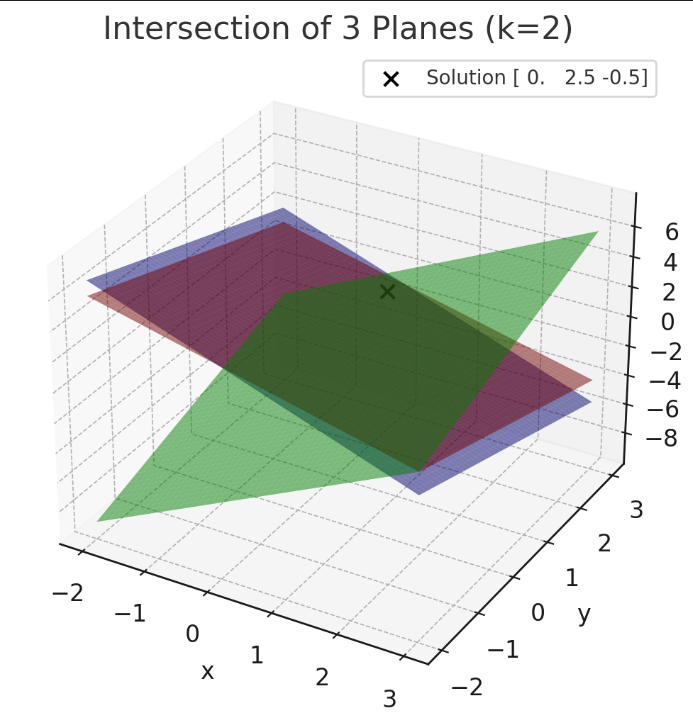
\includegraphics[width=0.75\linewidth]{figs/image.png}
        \caption{Image}
        \label{fig:placeholder}
\end{figure}
\end{document}
